\section{Formalized Process Description}

\crule

\subsection{2014- Integrating Plant and Process Information as a Basis for 
  Automated Plant Diagnosis Tasks}

\textbf{Reference:} \cite{arroyo2014integrating}

This paper presents concepts to classify, integrate, and facilitate the access 
to relevant data as a basis for automated plant diagnosis tasks.

Automated Fault Detection and Diagnosis (AFDD),
\begin{itemize}
  \item plant history,
  \item data trends,
  \item process states/dynamics,
  \item plant structure.
\end{itemize}


The behavior of plant disturbances is not simply conditioned by 
\ctextbf{structural knowledge} or \ctextbf{process sequences} 
but also by further \ctextbf{propagation-related factors (PRFs)}.

\begin{tikzpicture}
  \tikzstyle{textnode} = [rectangle, draw = black]
  \node[textnode] (n0) {\textbf{PRFs}};
  \node[textnode] (n1) [right = 2.5cm of n0] {\textbf{Knowledge model}}
    edge[<-] node[above] {\footnotesize(integrate into)} (n0);
\end{tikzpicture}

\textbf{Definition of the FPB:}
  \begin{itemize}
    \item \textbf{VDE/VDI 3682}
  \begin{itemize}
    \item Product:
    
\begin{tikzpicture}
      \node[draw = black, fill = red!80, 
        circle, 
        text width = .3cm, 
        align = center, 
        thick] (product) {\clanodetxt{P}};
    \end{tikzpicture}

    \item Process Operator:
    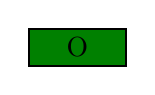
\begin{tikzpicture}
      \node[draw = black, 
        fill = green!50!black,
        rectangle,
        align = center,
        thick,
        text width = 1cm] 
        (proc_op) {\clanodetxt{O}};
    \end{tikzpicture}

    \item Technical Resource:
    \begin{tikzpicture}
      \node[draw = black,
        fill = black!50,
        rounded rectangle,
        align = center,
        thick,
        text width = 1cm] 
        (tech_res) {\clanodetxt{T}};
    \end{tikzpicture}

    \item Energy:
    \begin{tikzpicture}
      \node[draw = black,
        fill = blue!50,
        diamond,
        text width = .25cm,
        align = center,
        thick] (energy) {\clanodetxt{E}};
    \end{tikzpicture}

    \item Flow: 
    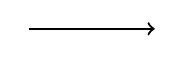
\begin{tikzpicture}
      \draw [->, thick] (0, 0) -- (1.6, 0);
    \end{tikzpicture}

    \item Utilization:
    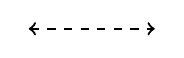
\begin{tikzpicture}
      \draw [<->, dashed, thick] (0, 0) -- (1.6, 0);
    \end{tikzpicture}

  \end{itemize}

  \item \textbf{Extension}
  \begin{itemize}
    \item Transport Resource:
    \begin{tikzpicture}
      \node[draw = black,
        fill = yellow!50,
        cylinder,
        align = center,
        shape border rotate=90,
        thick] (trans_res) {\clanodetxt{C}};
    \end{tikzpicture}

    \item Physical Link: 
    \begin{tikzpicture}
      \draw [dashed, red, thick] (0, 0) -- (1.6, 0);
    \end{tikzpicture}
  \end{itemize}
\end{itemize}